\chapter{Colloidal Nanocrystal Synthesis} \label{sec:CQDSynthesis} \index{Quantum Dot!Colloidal} \index{Quantum Dot!Synthesis}

	The colloidal chemistry has offered a remarkable amount of tools for creating nanostructures. In the past growing simple, spherical, monodisperse
	\glspl{NC} was the starting point of this research area, whereas nowadays various shapes, such as spheres, cubes, tetrapods,
	wires or rods can be engineered.
	The main advantages of the colloidal synthesis are:
	\begin{itemize}
		\itemsep 0pt
		\item High precision shape control of the crystal and multicomponent structures
		\item Good size adjustability, through which the optical properties of the material are determined
		\item Monodispersity of the \gls{NC}
		\item Low energy and low cost fabrication with a simple experimental setup
		\item Broad range of materials, including metals, semiconductors and magnetic materials can be synthesized at sub-20nm range
	\end{itemize}
	Due to the listed advantages, the colloidal \gls{NC} synthesis is the best candidate for commercial applications so far.
	
	\begin{REMARK}
		In the following section, we will be use some chemical terms. Their meaning can be looked up in the glossary on page \pageref{glossary}.
	\end{REMARK}
	
	\section{The synthesis}
		The colloidal \gls{NC} synthesis is a wet chemical method to create nanostructures. It is based on a three-component system composed
		of precursors, organic surfactants and solvents. Its basic idea is the controlled growth of a \gls{NC}, which is mainly depending on time. 	\\
		
		The basic apparatus of the synthesis is given in figure \ref{fig:LaMer}. It shows a reaction flask with thermometer and injection in form of a syringe.
		In praxis a heater is installed	around the lower part of the flask, to keep the solvent at a desired constant temperature.
		The procedure itself starts with the heating of a solvent funneled into the flask. The thermometer will indicate the temperature of the solvent,
		which is a key variable for a good growth process. Therefore it is important to control, as the reaction will have an influence on the temperature
		as well.
		Figure \ref{fig:LaMer} furthermore illustrates the stages of the synthesis using the traditional LaMer model by the U.S.-American chemist Victor LaMer.
		The nucleation process starts after the injection of the precursors into the flask, where they decompose and form monomers, which will cause the nucleation
		and growth of the \glspl{NC}. The size of the \gls{NC} is at this stage primarily determined by the time, i.e. the longer the reaction, the larger the
		crystals will grow.
		The energy required to decompose the precursors is provided by the solvent in the flask, either by thermal collisions or by a chemical reaction between the
		liquid medium and the precursors or by a combination of these two mechanisms \cite{Schmid}.
		Once monomer concentrations are sufficiently depleted, growth can proceed by Oswald ripening. Smaller particles combine with larger ones and cause therefore
		a lower concentration of particles in the solution.
		Unfortunately, the process is more complicated, as the model predicts. It does not hold for hot-injection schemes for instance,
		because nucleation, ripening and growth may almost occur concurrently \cite[p.5]{Klimov}. Furthermore the nucleation process
		does not have to start immediately after injection, but it is usually a single discrete event in time.
		In the following paragraph we will explain the variables that influence the reaction and their relationship to each other.
		
		As soon as the final size is reached, the reaction is stopped, by switching off the heating and cooling down the compound.
		After the reaction is stopped, the \glspl{NC} get washed to remove impurities from the reaction.
		
		\begin{figure}
			\centering
			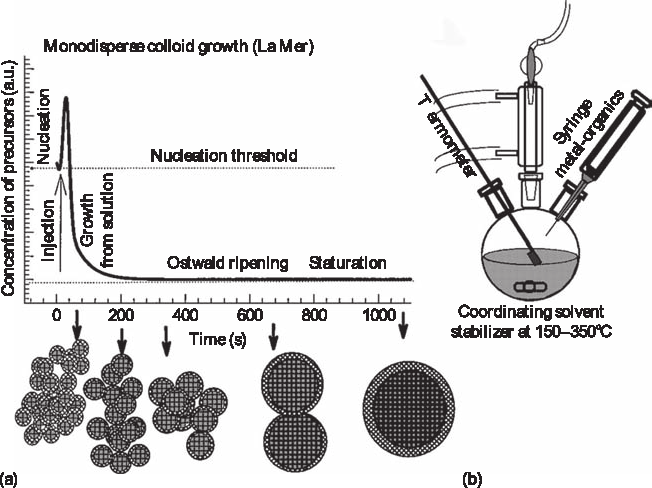
\includegraphics[width=0.5\textwidth]{Fig/LaMer.pdf}
			\caption{(a) Stages of the monodisperse \gls{NC} synthesis according to La Mer. (b) Basic apparatus used in the synthesis. {\scshape Source:} \cite[p.4]{Klimov}}
			\label{fig:LaMer}
		\end{figure}
		
	
	\section{Reaction conditions}
		Typically, finding the right conditions for a reaction is a very difficult task. For different materials, the conditions change and the reaction components
		have to be tailored exactly for this specific material. Hence finding an optimal set of conditions decides over the quality of the resulting \glspl{NC}.
		
		\paragraph{Duration of the particle growth} As mentioned, the duration of the process after injecting the precursors, determines the size of the particles.
		One might ask, when the right moment is to stop the synthesis, because the particles itself cannot be measured during the reaction. Due to this fact, the time
		to reach a desired size is determined empirically.
	
		\paragraph{Reaction temperature} The temperature is a critical factor for determining optimal crystal growth. 
		High reaction temperatures of 125�C-400�C are often needed to anneal out defects in the crystalline
		lattice to form highly crystalline particles \cite{Schmid}. In addition to that precursors have to withstand such high temperatures
		on the one hand and on the other hand temperatures need to be high enough, that precursors turn into monomers.
		This contradiction makes researchers to look for specific materials that fit the needed conditions.

		\paragraph{Concentration of surfactants} The choice of surfactants varies from case to case: a molecule that binds too strongly to the surface of the \gls{QD}
		is not suitable, as it would not allow the crystal to grow. On the other hand, a weakly coordinating molecule would yield large particles or aggregates. \\
	
		The combination of these conditions decides, if the final \gls{QD} is of poor or high quality. Especially for semiconductor \glspl{QD} a high luminescence
		efficiency is of great importance, since one would like to use the \glspl{NC} for example in solar cells.
		Therefore a high efficiency rate would increase the performance of the photovoltaic elements. This can be achieved by a proper control of surface chemistry,
		as this can eliminate midgap states associated with surface dangling bonds \cite{Talapin}.